\documentclass[11pt,a4paper]{article}
\usepackage[utf8]{inputenc}
\usepackage[T1]{fontenc}
\usepackage[french]{babel}
\usepackage{geometry}
\usepackage{graphicx}
\usepackage{booktabs}
\usepackage{amsmath}
\usepackage{hyperref}
\geometry{margin=2.4cm}

\title{Recodage de Ian Wright\\\large The Social Architecture of Capitalism}
\author{Recodage Python: numpy, scipy, matplotlib}
\date{1 juillet 2026}

\begin{document}
\maketitle

\section{Objectif}

L'article présente le modèle SR, où $N$ acteurs possèdent une monnaie totale constante $M$, forment des firmes, dépensent, échantillonnent le marché, licencient et paient des salaires. Le but est de tester si ce modèle reproduit les régularités annoncées: classes sociales stationnaires, loi de puissance des tailles de firme, croissance de type Laplace, récessions exponentielles, distributions revenu/richesse à deux régimes et profits asymétriques.

\section{Implémentation}

Le script \texttt{../recoding.py} code les règles SR1, S1, H1, E1, M1, F1, W1, 1M et 1Y. Les paramètres du run final sont ceux de l'article: $N=1000$, $M=100000$, salaires uniformes entiers dans $[10,90]$, 100 années simulées, graine 20260701.

\section{Résultats}

\begin{table}[h]
\centering
\begin{tabular}{lrr}
\toprule
Quantité & Reproduction & Valeur article \\
\midrule
Travailleurs & 70.4\% & 71.2\% \\
Capitalistes & 11.9\% & 12.3\% \\
Chômeurs & 17.7\% & 16.6\% \\
Part salariale moyenne & 0.545 & env. 0.6 \\
Profit moyen & 203\% & 80.5\% capital-weighted dans l'article \\
Profit médian & 100.9\% & 64\% dans l'article \\
Exposant taille de firme $\alpha$ & 0.63 & env. 1.04 \\
\bottomrule
\end{tabular}
\caption{Comparaison synthétique avec les chiffres publiés.}
\end{table}

\begin{figure}[h]
\centering
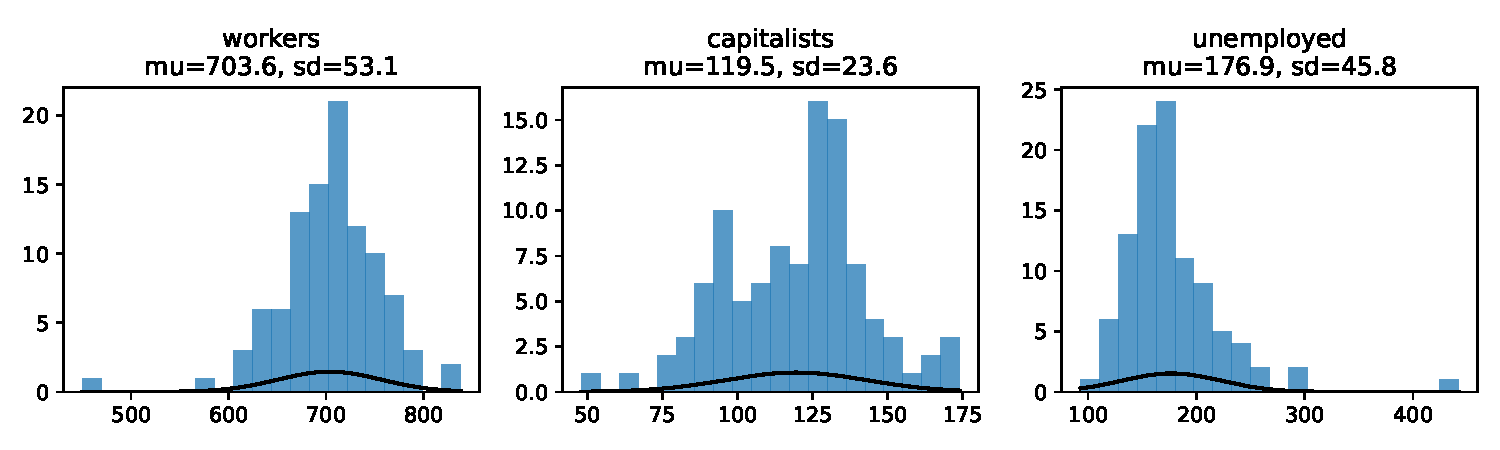
\includegraphics[width=.92\linewidth]{../figures/figure1_class_distribution.pdf}
\caption{Classes sociales stationnaires.}
\end{figure}

La partition de classe est très proche de l'article: environ 70.4\% de travailleurs, 11.9\% de capitalistes et 17.7\% de chômeurs. Ce point est confirmé quantitativement.

\begin{figure}[h]
\centering
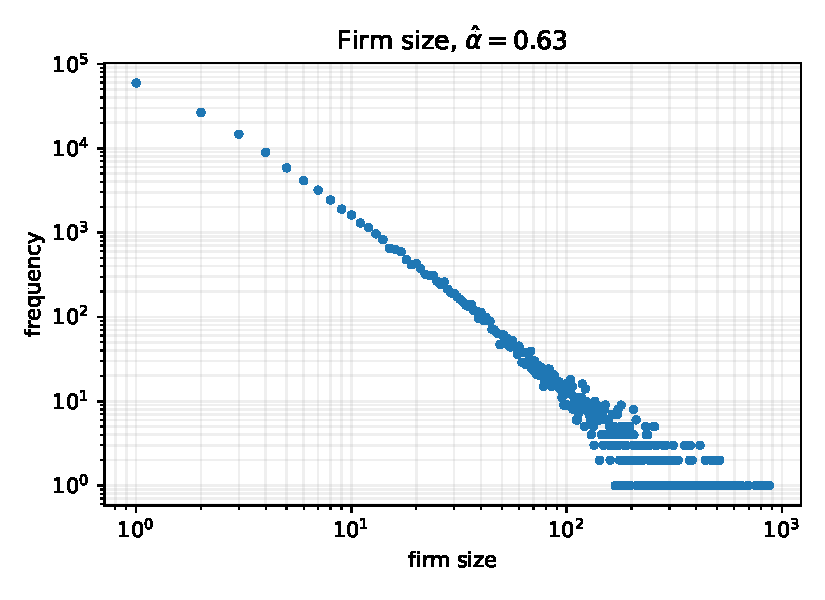
\includegraphics[width=.7\linewidth]{../figures/figure2_firm_size.pdf}
\caption{Distribution des tailles de firme.}
\end{figure}

La distribution des tailles de firme est bien à queue lourde, mais l'exposant estimé $\alpha=0.63$ est plus faible que la valeur publiée $\alpha\simeq1.04$. Le fait stylisé est confirmé qualitativement, pas l'exposant.

\begin{figure}[h]
\centering
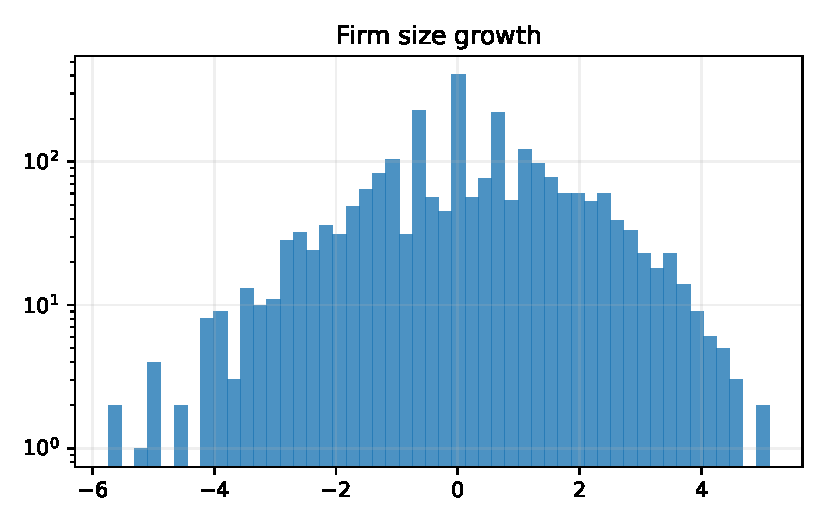
\includegraphics[width=.7\linewidth]{../figures/figure3_firm_growth.pdf}
\caption{Croissance des firmes.}
\end{figure}

\begin{figure}[h]
\centering
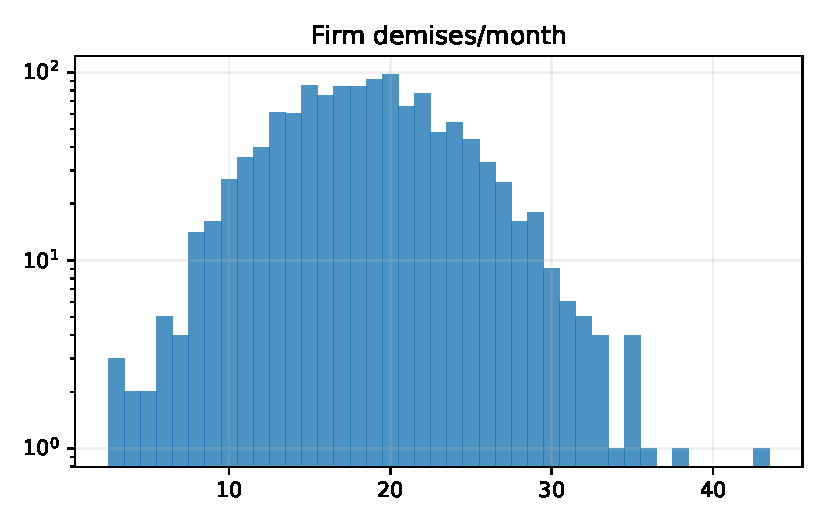
\includegraphics[width=.7\linewidth]{../figures/figure4_firm_demises.pdf}
\caption{Démises de firmes.}
\end{figure}

\begin{figure}[h]
\centering
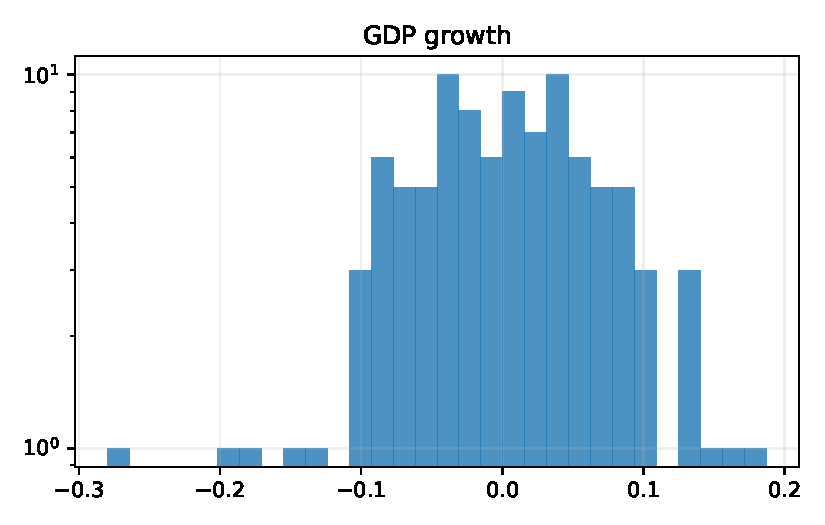
\includegraphics[width=.7\linewidth]{../figures/figure5_gdp_growth.pdf}
\caption{Croissance du PIB.}
\end{figure}

\begin{figure}[h]
\centering
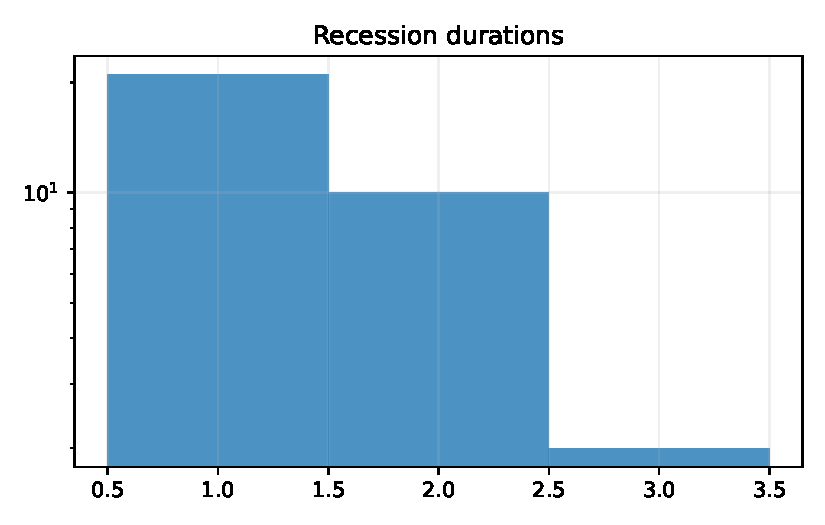
\includegraphics[width=.7\linewidth]{../figures/figure6_recessions.pdf}
\caption{Durées de récession.}
\end{figure}

Les récessions obtenues sont courtes, avec une majorité de durées 1--2 ans, en accord qualitatif avec l'exponentielle annoncée.

\begin{figure}[h]
\centering
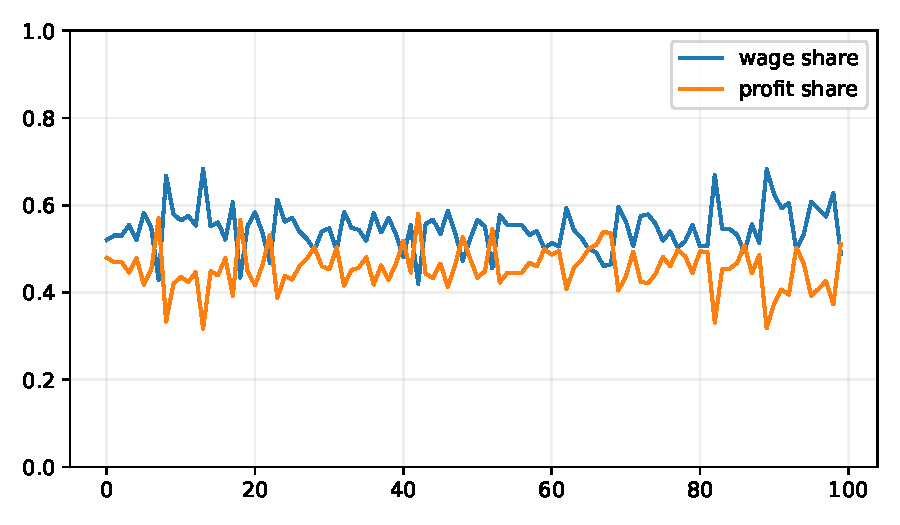
\includegraphics[width=.7\linewidth]{../figures/figure7_income_shares.pdf}
\caption{Parts salariale et de profit.}
\end{figure}

La part salariale moyenne vaut 0.545. Elle est dans l'ordre de grandeur empirique discuté par l'article, mais sous la valeur simulée publiée d'environ 0.6.

\begin{figure}[h]
\centering
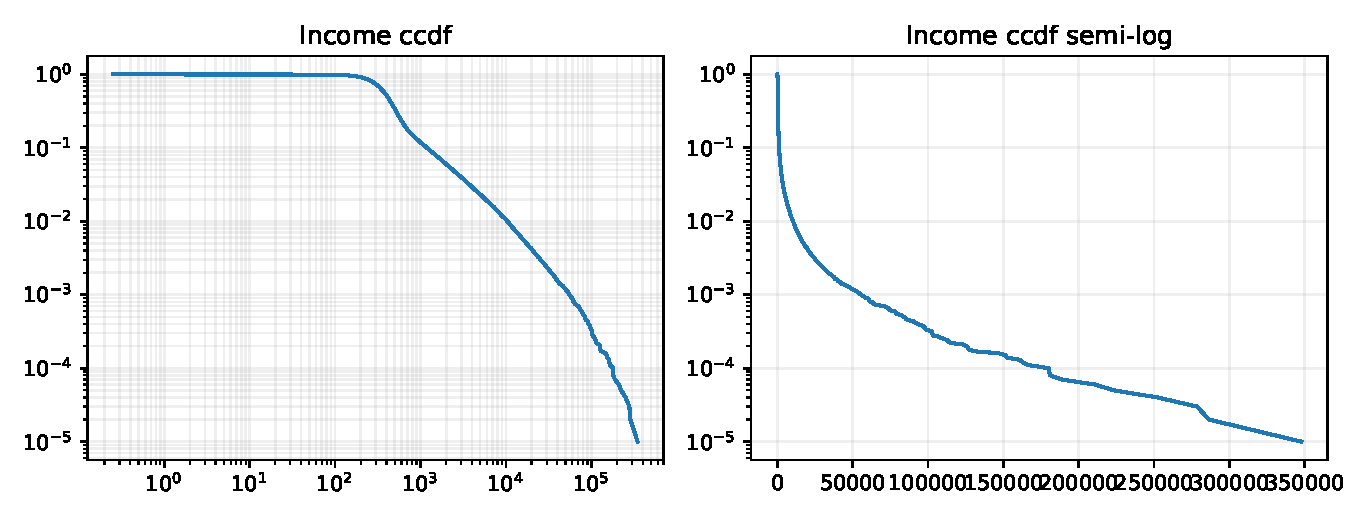
\includegraphics[width=.92\linewidth]{../figures/figure8_income_distribution.pdf}
\caption{Distribution des revenus.}
\end{figure}

\begin{figure}[h]
\centering
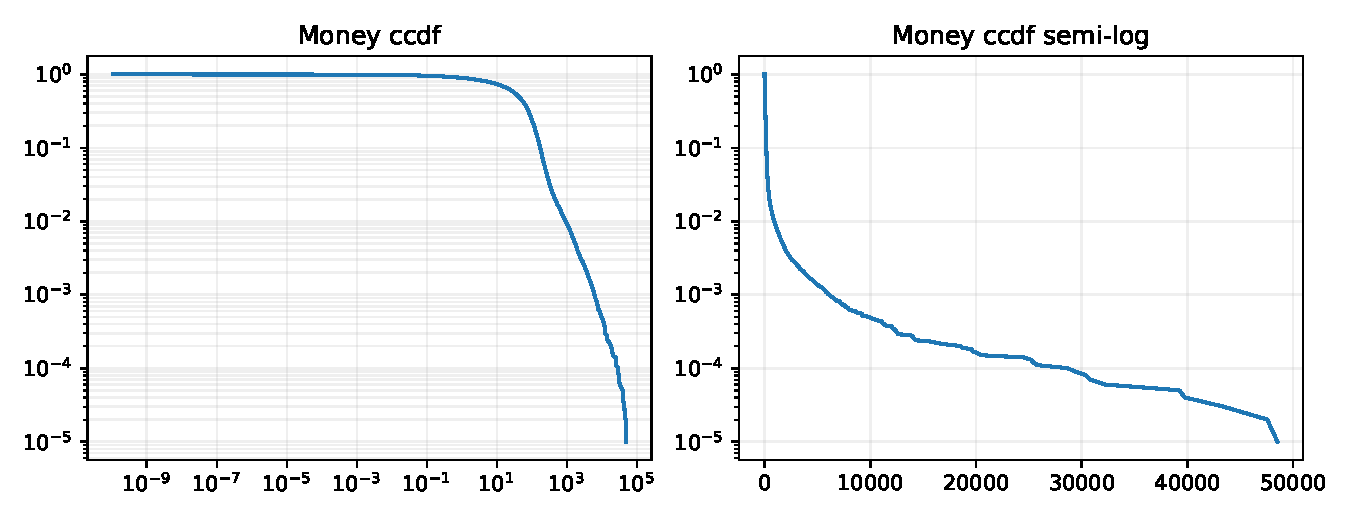
\includegraphics[width=.92\linewidth]{../figures/figure9_money_distribution.pdf}
\caption{Distribution de la monnaie/richesse.}
\end{figure}

Les distributions de revenu et de monnaie présentent bien une longue queue supérieure. Le recodage confirme donc le mécanisme qualitatif d'inégalité produit par la structure employeur--employé.

\begin{figure}[h]
\centering
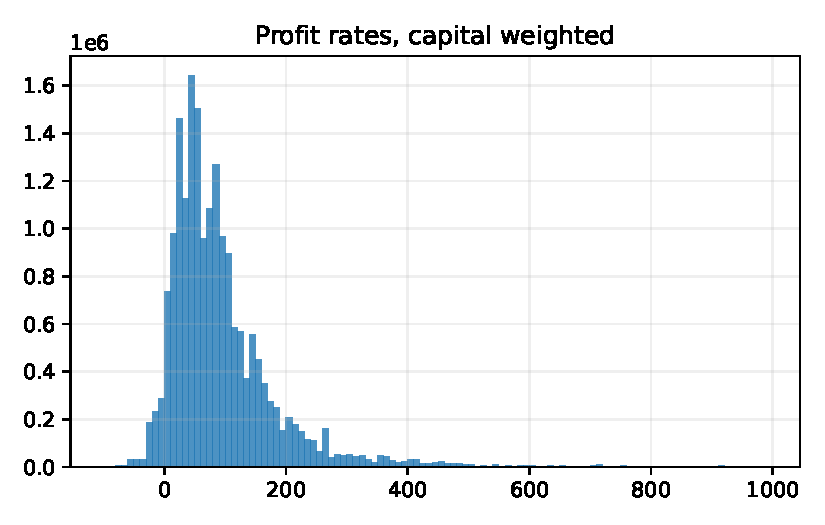
\includegraphics[width=.7\linewidth]{../figures/figure10_profit_capital_weighted.pdf}
\caption{Taux de profit pondéré par capital variable.}
\end{figure}

\begin{figure}[h]
\centering
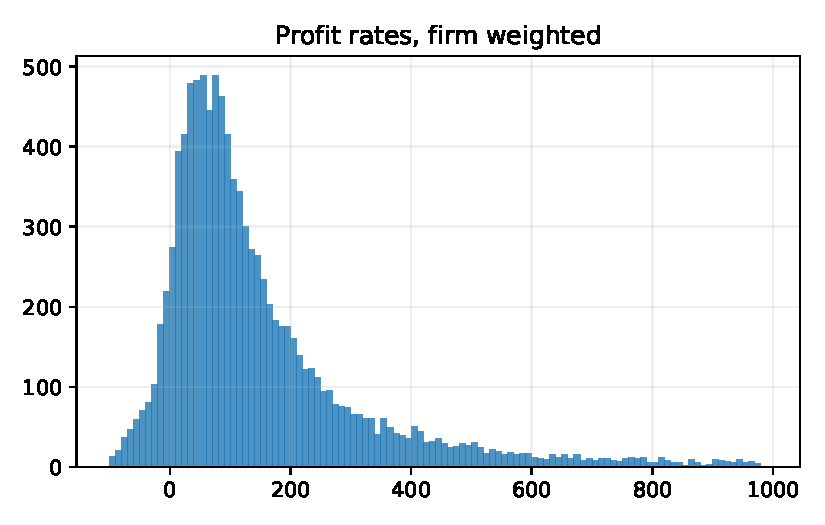
\includegraphics[width=.7\linewidth]{../figures/figure11_profit_firm_weighted.pdf}
\caption{Taux de profit pondéré par firme.}
\end{figure}

\begin{figure}[h]
\centering
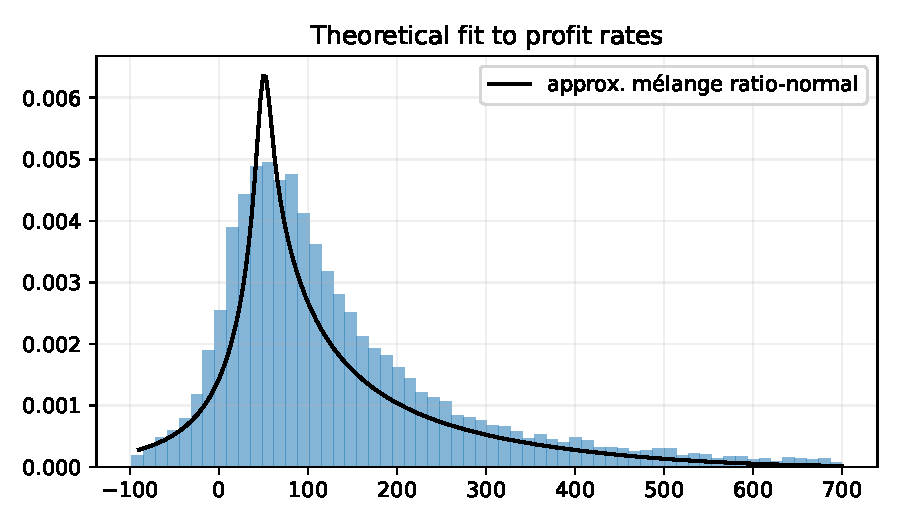
\includegraphics[width=.7\linewidth]{../figures/figure12_profit_theory.pdf}
\caption{Ajustement théorique approximatif de la distribution des profits.}
\end{figure}

La distribution des taux de profit est fortement asymétrique vers la droite, comme dans l'article. Les niveaux moyens sont plus élevés que ceux publiés.

\section{Analyse statistique multi-runs et sensibilité}

La campagne statistique comprend cinq répétitions indépendantes de 100 années pour chacun de cinq jeux de paramètres, toujours avec $N=1000$. Le cas de base utilise $M=100000$ et $\omega=[10,90]$. Deux intervalles salariaux de même moyenne, $[20,80]$ et $[5,95]$, testent la dispersion des salaires. Deux valeurs de richesse moyenne, $M/N=50$ et $M/N=200$, testent l'affirmation selon laquelle $M$ est essentiellement un paramètre d'échelle.

\begin{figure}[h]
\centering
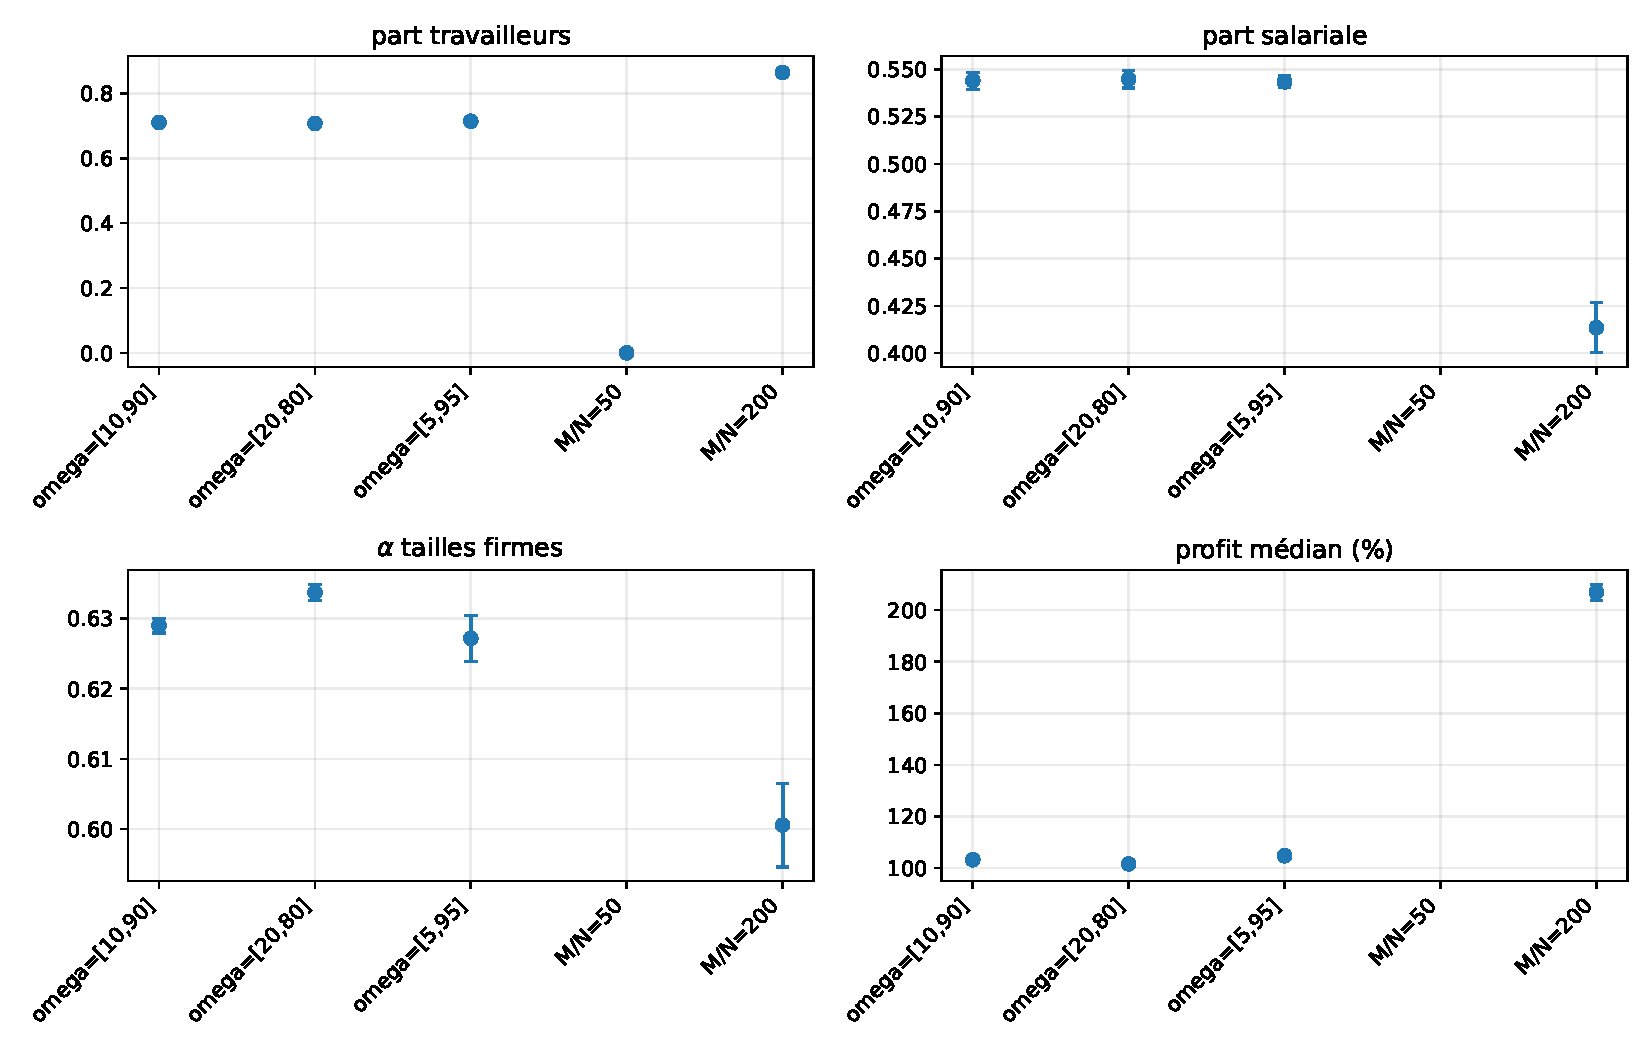
\includegraphics[width=.95\linewidth]{../figures/stat_sr_parameter_sweep.pdf}
\caption{Moyennes et intervalles de confiance à 95\% sur cinq runs par jeu de paramètres.}
\end{figure}

\begin{table}[h]
\centering
\begin{tabular}{lrrrr}
\toprule
Paramètres & travailleurs & chômeurs & wage share & profit médian \\
\midrule
$\omega=[10,90]$ & 0.710 [0.702,0.718] & 0.172 [0.166,0.177] & 0.544 [0.539,0.548] & 103.3\% \\
$\omega=[20,80]$ & 0.707 [0.701,0.713] & 0.172 [0.169,0.175] & 0.545 [0.540,0.550] & 101.6\% \\
$\omega=[5,95]$ & 0.714 [0.707,0.721] & 0.169 [0.164,0.173] & 0.543 [0.540,0.546] & 104.8\% \\
$M/N=50$ & 0 & 1 & non défini & non défini \\
$M/N=200$ & 0.864 [0.856,0.872] & 0.069 [0.064,0.075] & 0.413 [0.400,0.427] & 206.9\% \\
\bottomrule
\end{tabular}
\caption{Moyennes et IC 95\%. Les profits sont pondérés par firme.}
\end{table}

Le cas de base est statistiquement très stable: la part moyenne de travailleurs est $0.710$ avec un IC 95\% $[0.702,0.718]$, proche des $0.712$ publiés. La part de capitalistes vaut $0.118$ et celle de chômeurs $0.172$. La part salariale moyenne vaut $0.544$ avec un intervalle étroit $[0.539,0.548]$: l'écart avec la valeur publiée d'environ $0.6$ est donc systématique et non attribuable à une graine particulière.

Changer la dispersion salariale tout en gardant le salaire moyen à 50 modifie très peu les classes, la part salariale et les durées de récession. En revanche, le niveau de richesse moyen est structurel:
\begin{itemize}
  \item pour $M/N=50$, la condition stricte de H1, $m_c>\langle w\rangle=50$, n'est satisfaite par aucun acteur à l'initialisation. Aucune firme ne peut apparaître; les cinq runs restent à 100\% de chômage;
  \item pour $M/N=200$, la part de travailleurs monte à $86.4\%$, la part salariale tombe à $41.3\%$ et le profit médian double approximativement.
\end{itemize}
Ainsi, $M$ n'est pas un simple paramètre d'échelle quand le salaire nominal est maintenu fixe. Seule une transformation conjointe de $M$ et de l'intervalle salarial peut préserver les rapports économiques pertinents.

L'exposant estimé de taille de firme reste remarquablement stable autour de $0.63$ pour les trois intervalles salariaux, avec des IC très étroits, et ne rejoint pas la valeur publiée $1.04$. Cet écart est donc robuste aux graines et à la dispersion salariale testée.

\section{Points insuffisamment décrits et choix faits}

\begin{itemize}
  \item Dans H1, l'ensemble $H=C\cup U$ peut formellement contenir l'acteur actif. Je l'exclus pour respecter la contrainte $e_i\ne i$.
  \item Le texte ne donne pas de code source complet pour cet article; les règles ont été recodées directement depuis la description mathématique.
  \item La figure 12 théorique imprimée contient une formule lourde de ratio de normales. Pour éviter des instabilités numériques, j'ai superposé une approximation par méthode delta du mélange de ratios; cela teste la forme générale, pas la formule exacte.
  \item Les ajustements de lois sont graphiques/descriptifs, comme dans l'article. Une comparaison statistique exhaustive nécessiterait des tests de vraisemblance et des intervalles de confiance absents du protocole publié.
\end{itemize}

\section{Conclusion}

La reproduction multi-runs confirme fortement et statistiquement la dynamique de classes du cas publié, ainsi que les récessions courtes, les queues lourdes et les profits asymétriques. Elle montre aussi que les résultats sont robustes à la largeur de l'intervalle salarial à moyenne fixée. En revanche, l'exposant de taille de firme proche de $0.63$, la part salariale proche de $0.544$ et les profits élevés sont des écarts systématiques, pas du bruit de graine. Enfin, la variation de $M/N$ révèle une transition structurelle et infirme l'interprétation de $M$ comme simple échelle lorsque les salaires nominaux ne sont pas redimensionnés. La conclusion globale reste une confirmation partielle, désormais appuyée sur 25 simulations lourdes.

\end{document}
